\input{estilo}
% La tabla de la pizarra: tres columnas, ID, MSG y VISIBILITY_TO, y dos filas
% vacías.
\begin{document}
\begin{figura}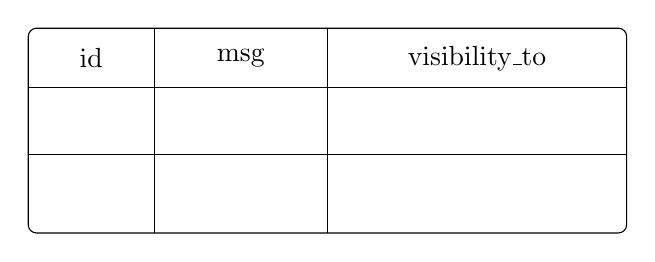
\begin{tikzpicture}
  \draw[rounded corners=3pt] (0,0) rectangle (7.6,-2.6);
  \draw (1.6,0) -- (1.6,-2.6) (3.8,0) -- (3.8,-2.6);
  \draw (0,-0.75) -- (7.6,-0.75) (0,-1.6) -- (7.6,-1.6);
  \foreach \x/\t in {0.8/id, 2.7/msg, 5.7/visibility\_to} \node at (\x,-0.38) {\t};
\end{tikzpicture}\end{figura}
\end{document}
